\documentclass[a4paper,10pt]{article}
\usepackage[a4paper, total={5.5in, 8.5in}]{geometry}	% define width and height of text part of a page
\usepackage[utf8x]{inputenc}
\usepackage{array}
\usepackage[pdftex]{graphicx}
\usepackage{listings}
\usepackage{enumitem}
\usepackage{color, colortbl}
\usepackage{longtable}
\usepackage{float}
\usepackage[ddmmyyyy]{datetime}
\usepackage[compact]{titlesec}		% The 'compact' argument reduces spacing before and after headings

% Start ---- Fix for bug in issue 2.10.1 of titlesec package
\usepackage{etoolbox}

\makeatletter
\patchcmd{\ttlh@hang}{\parindent\z@}{\parindent\z@\leavevmode}{}{}
\patchcmd{\ttlh@hang}{\noindent}{}{}{}
\makeatother
% End ---- Fix for bug in issue 2.10.1 of titlesec package

\usepackage{verbatim}
\usepackage{fancyhdr}
\usepackage{datatool}	% Management of external databases
\usepackage{chngcntr}	% Management of figure and table numberings
\usepackage{pdflscape}	% Provides 'landscape mode' for selected pages
\usepackage{hyperref}


%---------------------------------------------
% Management of Figure and Table Numbering
%---------------------------------------------
\counterwithin{figure}{section}
\counterwithin{table}{section}

%---------------------------------------------
% Management of Captions (options interact with each other in unpredictable ways)
%---------------------------------------------
\usepackage[labelfont=bf]{caption}	% The caption label for tables and figures is bolded
\setlength{\abovecaptionskip}{2pt}	% Bring caption close to figure or table
\setlength{\belowcaptionskip}{-8pt}	% Bring caption close to text after it
\renewcommand{\figurename}{Fig.}	% The caption label for figures is: "Fig."
%\captionsetup[table]{singlelinecheck=off,justification=raggedright}	% Justify the table captions to the left
\captionsetup[table]{position=bottom,skip=-1pt}	% controls spacing between caption and table
%\captionsetup[figure]{position=bottom,skip=40pt}	

\pagestyle{fancy}

%------------------------------------------------------------------------------------------
% Directories holding image files:
% - Figures from CORDET FW Project
% - Figures from CHEOPS Project
% - Figures from FW Profile Project
%------------------------------------------------------------------------------------------
\graphicspath{ {../../images/} {../../../cr/images/} {../../../sm/images/} }	

%---------------------------------------------
% Paragraph Layout
%---------------------------------------------
\setlength{\parindent}{0in}			% No indentation on first line of a new paragraph

%---------------------------------------------
% Table Layout
%---------------------------------------------
\setlength{\extrarowheight}{1.5pt}	% Add vertical space at a table row
 
 %---------------------------------------------
% Management of changes
%---------------------------------------------
\newcommand{\chg}[1]{{\color{black}{#1}}{}} 
\newcommand{\chgAB}[1]{{\color{black}{#1}}{}} 	% Changes in version 1.2
\newcommand{\chgB}[1]{{\color{black}{#1}}{}} 	% Changes in version 2
\newcommand{\chgC}[1]{{\color{black}{#1}}{}} 	% Changes in version 3
\newcommand{\chgCA}[1]{{\color{black}{#1}}{}} 	% Changes in imported event table
\newcommand{\chgD}[1]{{\color{black}{#1}}{}} 	% Changes in version 4
\newcommand{\chgDA}[1]{{\color{black}{#1}}{}} 	% Changes in version 4.1
\newcommand{\chgE}[1]{{\color{black}{#1}}{}} 	% Changes in version 5
\newcommand{\chgF}[1]{{\color{black}{#1}}{}} 	% Changes in version 6
\newcommand{\chgFA}[1]{{\color{black}{#1}}{}} 	% Changes in version 6.1
\newcommand{\chgFB}[1]{{\color{black}{#1}}{}} 		% Changes in version 6.2
\newcommand{\chgFC}[1]{{\color{black}{#1}}{}} 		% Changes in version 6.3
\newcommand{\chgFD}[1]{{\color{black}{#1}}{}} 		% Changes in version 6.4
\newcommand{\chgG}[1]{{\color{black}{#1}}{}} 		% Changes in version 7
\newcommand{\chgGA}[1]{{\color{black}{#1}}{}} 		% Changes in version 7.1
\newcommand{\chgH}[1]{{\color{red}{#1}}{}} 		% Changes in version 8

%------------------------------------------------------------------------------------------
% Management of Headings
%------------------------------------------------------------------------------------------
% Define spacing to the left, before and after a subsection heading
%\titlespacing\subsubsection{8pt}{12pt plus 4pt minus 2pt}{-10pt plus 0pt minus 0pt}
\titlespacing\subsubsection{0pt}{5pt}{0pt}
\titlespacing\subsection{0pt}{5pt}{0pt}

% Introduce a page break before each section
\let\stdsection\section
\renewcommand\section{\newpage\stdsection}

%---------------------------------------------
% Definition of custom properties
%---------------------------------------------
\newcommand{\docIssue}{0.1}						% issue number
\newcommand{\docRefNumber}{PP-DF-COR-0003}		% document reference number

%---------------------------------------------
% Headers and Footers
%---------------------------------------------
\renewcommand{\headrulewidth}{0.4pt}
\renewcommand{\footrulewidth}{0.4pt}

\lhead{\docRefNumber{}}
\chead{}
\rhead{Revision \docIssue{}}
\lfoot{\textcopyright2014 P\&P Software GmbH. All Rights Reserved.}
\cfoot{\vspace{5mm}
%{\color{red}\verbatiminput{../commercial/LicensedTo.txt}}}
\rfoot{\thepage}
\renewcommand{\headrulewidth}{0.4pt}
\renewcommand{\footrulewidth}{0.4pt}

%---------------------------------------------
% Management of lists
%---------------------------------------------
\setlist{nolistsep}								% No extra vertical space around a list		
\newenvironment{fw_itemize}						% Control spacing between items in a list
{\begin{itemize}
  \setlength{\itemsep}{1mm}
  \setlength{\parskip}{0pt}
  \setlength{\parsep}{0pt}}
{\end{itemize}}

\newenvironment{fw_enumerate}					% Control spacing between items in an enumeration
{\begin{enumerate}
  \setlength{\itemsep}{1mm}
  \setlength{\parskip}{0pt}
  \setlength{\parsep}{0pt}}
{\end{enumerate}}

\newenvironment{fw_description}					% Control spacing between items in a description
{\begin{description}
  \setlength{\itemsep}{1mm}
  \setlength{\parskip}{5pt}			% Line spacing between paragraphs in an item
  \setlength{\parsep}{0pt}}
{\end{description}}

%---------------------------------------------
% Definition of colours
%---------------------------------------------
\definecolor{dkgreen}{rgb}{0,0.6,0}
\definecolor{gray}{rgb}{0.5,0.5,0.5}
\definecolor{light-gray}{gray}{0.85}
\definecolor{mauve}{rgb}{0.58,0,0.82}
\definecolor{lightblue}{RGB}{128,179,255}
\definecolor{lbcolor}{rgb}{0.9,0.9,0.9}

%------------------------------------------------------
% Management of text which is conditionally included
%------------------------------------------------------
\newcommand{\umOnly}[1]{#1}
\renewcommand{\umOnly}[1]{} %Comment out this whole line to suppress exclusion.

\newcommand{\iaswOnly}[1]{#1}
%\renewcommand{\iaswOnly}[1]{} %Comment out this whole line to suppress exclusion.

%---------------------------------------------
% Define Environment for Requirement Tables 
% Par #1: The string identifying the requirement category
% Par #2: The table caption
%---------------------------------------------
\newenvironment{cr_req}[2]
{
\begin{longtable}{|l|p{10.4cm}|}
\caption{#2} \\
\hline
\rowcolor{light-gray}
\textbf{Req. ID} & \textbf{Requirement Text}\\
\hline\hline
\endfirsthead
\rowcolor{light-gray}
\textbf{Req. ID} & \textbf{Requirement Text}\\
\hline\hline
\endhead
\DTLforeach*[\DTLiseq{\cat}{#1}]{dbReq}{\cat=Cat,\id=N,\type=Type,\ver=Ver,\reqText=Text}
{\DTLiffirstrow{}{\\\hline}\cat-\id/\type\ver & \reqText}\\\hline
}
{\end{longtable}}

%---------------------------------------------
% Define Environment for IASW Command Tables 
% Par #1: The string identifying the cmd name
% Par #2: The table caption
%---------------------------------------------
\newenvironment{ch_cmd}[2]
{
\begin{longtable}{|l|p{9.6cm}|}
\caption{#2} \label{tab:#1} \\
\hline
\rowcolor{light-gray}
\DTLforeach*{dbCmd}{\att=Attribute,\attValue=#1}
{\DTLiffirstrow{}{\\\hline}\att & \attValue}\\\hline
}
{\end{longtable}}

%---------------------------------------------
% Define Environment for SEM Command Tables 
% Par #1: The string identifying the cmd name
% Par #2: The table caption
%---------------------------------------------
\newenvironment{sem_cmd}[2]
{
\begin{longtable}{|l|p{9.6cm}|}
\caption{#2} \label{tab:#1} \\
\hline
\rowcolor{light-gray}
\DTLforeach*{dbSemCmd}{\attSem=Attribute,\attValueSem=#1}
{\DTLiffirstrow{}{\\\hline}\attSem & \attValueSem}\\\hline
}
{\end{longtable}}

%---------------------------------------------
% Define Environment for Report Tables 
% Par #1: The string identifying the rep name
% Par #2: The table caption
%---------------------------------------------
\newenvironment{ch_rep}[2]
{
\begin{longtable}{|l|p{9.6cm}|}
\caption{#2} \label{tab:#1}\\
\hline
\rowcolor{light-gray}
\DTLforeach*{dbRep}{\att=Attribute,\attValue=#1}
{\DTLiffirstrow{}{\\\hline}\att & \attValue}\\\hline
}
{\end{longtable}}

%---------------------------------------------
% Define Environment for Parameter Tables 
% Par #1: The string identifying the proc or algo name
% Par #2: The table caption
%---------------------------------------------
\newenvironment{pa_par}[2]
{
\begin{longtable}{|c|l|>{\raggedright\arraybackslash}p{4.0cm}|p{5.0cm}|}
\caption{#2} \label{tab:#1}\\
\hline
\rowcolor{light-gray}
\textbf{N} & \textbf{Name} & \textbf{Description} & \textbf{Constraints} \\
\hline\hline
\endfirsthead
\rowcolor{light-gray}
\textbf{N} & \textbf{Name} & \textbf{Description} & \textbf{Constraints} \\
\hline\hline
\endhead
\DTLforeach*[\DTLiseq{\paName}{#1}]{dbPar}{\paName=ProcAlgoName,\paN=ParN,\paPar=ParName,\paDesc=ParDesc,\paConst=ParConstraints}
{\DTLiffirstrow{}{\\\hline}\paN & \texttt{\paPar} & \paDesc & \paConst}\\\hline
}
{\end{longtable}}


%---------------------------------------------
% Options for the code listing boxes
%---------------------------------------------
\lstset{ 
  language=C,                % the language of the code
  aboveskip=\bigskipamount,			% vertical space above listing box
  belowskip=0pt,					% vertical space below listing box
  basicstyle=\scriptsize\ttfamily,    % use small size and mono-space font
  numbers=left,                   % where to put the line-numbers
  numberstyle=\tiny\color{gray},  % the style that is used for the line-numbers
  stepnumber=1,                   % the step between two line-numbers. If it's 1, each line 
                                  % will be numbered
  numbersep=5pt,                  % how far the line-numbers are from the code
  backgroundcolor=\color{lbcolor},      % choose the background color. You must add \usepackage{color}
  showspaces=false,               % show spaces adding particular underscores
  showstringspaces=false,         % underline spaces within strings
  showtabs=false,                 % show tabs within strings adding particular underscores
  frame=single,                   % adds a frame around the code
  rulecolor=\color{black},        % if not set, the frame-color may be changed on line-breaks within not-black text (e.g. commens (green here))
  tabsize=2,                      % sets default tabsize to 2 spaces
  captionpos=b,                   % sets the caption-position to bottom
  breaklines=true,                % sets automatic line breaking
  breakatwhitespace=false,        % sets if automatic breaks should only happen at whitespace
  title=\lstname,                   % show the filename of files included with \lstinputlisting;
                                  % also try caption instead of title
  keywordstyle=\color{blue},          % keyword style
  commentstyle=\color{dkgreen},       % comment style
  stringstyle=\color{mauve},         % string literal style
  escapeinside={\%*}{*)},            % if you want to add a comment within your code
  morekeywords={*,...}               % if you want to add more keywords to the set
}
%---------------------------------------------
% Import tables with requirements and adaptation points
%---------------------------------------------
\DTLloaddb{dbServ}{CheopsServices.csv}
\DTLloaddb{dbSemServ}{SemServices.csv}
\DTLloaddb{dbSemCmd}{SemCmds.csv}
\DTLloaddb{dbReq}{CheopsIaswReq.csv}
\DTLloaddb{dbFail}{CheopsCmdFailCodes.csv}
\DTLloaddb{dbEvt}{CheopsEvtRep.csv}
\DTLloaddb{dbCmd}{CheopsCmds.csv}
\DTLloaddb{dbRep}{CheopsReps.csv}
\DTLloaddb{dbHkRep}{CheopsHkReps.csv}
\DTLloaddb{dbPar}{CheopsAlgoProcPar.csv}

%---------------------------------------------
% Pdf Properties
%---------------------------------------------
\hypersetup
{
    pdfauthor={Alessandro Pasetti},
    pdfsubject={This document specifies the PUS Extension of the CORDET Framework},
    pdftitle={PUS Extension of the CORDET Framework},
    pdfkeywords={PUS, CORDET}
}

%---------------------------------------------
% Title Page
%---------------------------------------------
\title{\textsc{The CORDET Framework} \\ \textsc{- PUS Extension -}}
\author{Alessandro Pasetti \& TBD}
\date{Created on: \today{}, at: \currenttime{}}

\begin{document}
\maketitle

\begin{center}
Revision \docIssue{}\\
\docRefNumber{}
\end{center}

\vspace{1cm}

\begin{center}
P\&P Software GmbH \\
High Tech Center 1 \\
8274 T\"{a}gerwilen (CH)\\
\vspace{2mm}
Web site: \url{www.pnp-software.com}\\
E-mail: \href{mailto:pnp-software@pnp-software.com}{\nolinkurl{pnp-software@pnp-software.com}} 
\end{center}

\vspace{0.5cm}

\begin{table}[ht]
\begin{center}
\begin{tabular}{p{11.7cm}}
\\
\hline
\end{tabular}
\end{center}
\end{table}
\begin{abstract}
This document specifies the PUS Extension of the CORDET Framework. The CORDET Framework is a software framework for service-oriented embedded applications. The service concept of the CORDET Framework is the same as the service concept of the Packet Utilization Standard or PUS. The PUS is an application-level interface standard for space-based distributed systems.

The PUS pre-defines a number of services. This document extends the CORDET Framework to support a subset of those services. The document specifies the components which implements them. The components are specified by providing their behavioural model. The behavioural models are defined using the FW Profile.

\end{abstract}
\begin{table}[ht]
\begin{center}
\begin{tabular}{p{11.7cm}}
\\
\hline
\end{tabular}
\end{center}
\end{table}


\newpage
\vspace*{\fill}
\begin{center}
No part of this publication may be reproduced, transmitted, transcribed, stored in any retrieval system, or translated into any language by any means without express prior written permission of P\&P Software GmbH.
\end{center}

\begin{center}
Copyright \textcopyright 2014 P\&P Software GmbH. All Rights Reserved. 
\end{center}
\vspace*{\fill}

%---------------------------------------------
% Table of Contents
%---------------------------------------------
\newpage
\tableofcontents

\newpage
\listoffigures
\listoftables

\newpage

%---------------------------------------------
% Adjust distance between paragraphs (this cannot be done earlier or it also affects the TOC)
%---------------------------------------------
\setlength{\parskip}{3mm}						% Set distance between paragraphs

%==========================================================================================
\section{Change History}

This section lists the changes made in the current and previous revisions. Changes are classified according to their type. The change type is identified in the second column in the table according to the following convention:

\begin{fw_itemize}
\item "\textbf{E}": Editorial or stylistic change
\item "\textbf{L}": Clarification of existing text
\item "\textbf{D}": A requirement has in whole or in part been deleted
\item "\textbf{C}": A requirement has been modified
\item "\textbf{N}": A new requirement has been introduced
\item "\textbf{T}": A TBD or TBC has been resolved
\end{fw_itemize}

Text which is new or has been modified in the current revision is in red font. If a figure has been modified, then its caption is in red font. Section header numbers do not change from one revision to the next (but new sections may, of course, be introduced). However, figure and table numbers may change and these changes are not tracked. Changes in the appendices are not tracked as they are consequences of changes in the main body of the document.

\begin{longtable}{|c|c|p{10cm}|}
\caption{Detailed List of Changes in Issue 0.1} \\
\hline
\rowcolor{light-gray}
\textbf{Sec} & \textbf{Type} & \textbf{Description of Change} \\
\hline\hline
\endfirsthead
\rowcolor{light-gray}
\textbf{Sec} & \textbf{Type} & \textbf{Description of Change} \\
\hline\hline
\endhead
n.a. & L & This is the first release of this document \\
\hline
\end{longtable}






\newpage

%==========================================================================================
\section{Applicable and Reference Documents}

The documents in table \ref{tab:appDoc} form an integral part of the present document. The documents in table \ref{tab:refDoc} are referenced in the present document and are for information only.

\begin{longtable}{|c|p{11cm}|}
\caption{Applicable Documents} \label{tab:appDoc}\\
\hline
\rowcolor{light-gray}
\textbf{ID} & \textbf{Title, Reference Number, Revision Number} \\
\hline\hline
\endfirsthead
\rowcolor{light-gray}
\textbf{ID} & \textbf{Title, Reference Number, Revision Number} \\
\hline\hline
\endhead
AD-1 & The CORDET Framework - Specification, PP-DF-COR-00002, Revision 1.6, P\&P Software GmbH, Switzerland, 2012, Available from: \url{www.pnp-software.com/cordetfw} \\
\hline
AD-2 & The Framework Profile, PP-DF-COR-00001, Revision 1.3, P\&P Software GmbH, Switzerland, 2012, Available from: \url{www.pnp-software.com/fwprofile} \\
\hline
AD-3 & Ground Systems and Operations – Telemetry and Telecommand Packet Utilization Standard, ECSS-E-70-41C, April 2016, European Cooperation for Space Standardization (ECSS) \\
\hline
\end{longtable}

\begin{longtable}{|c|p{11cm}|}
\caption{Reference Documents} \label{tab:refDoc}\\
\hline
\rowcolor{light-gray}
\textbf{ID} & \textbf{Title, Reference Number, Revision Number} \\
\hline\hline
\endfirsthead
\rowcolor{light-gray}
\textbf{ID} & \textbf{Title, Reference Number, Revision Number} \\
\hline\hline
\endhead
RD-1 & The CORDET Framework Project Web Site Profile, \url{www.pnp-software.com/cordetfw} \\
\hline
\end{longtable}


\newpage


%==========================================================================================
\section{Introduction}
The CORDET Framework is a software framework for service-oriented embedded applications. It is specified in AD-1 as a set of components to manage the services which an application provides to other applications and uses from other applications. A C-language implementation of this specification is available from RD-1.

The CORDET Framework only covers the management of generic services but does not specify any concrete services. The service concept of the CORDET Framework is the same as the service concept of the \textit{Packet Utilization Standard} (PUS). The PUS is an application-level interface standard for space-based distributed systems. It is defined in AD-3.

The PUS pre-defines a number of services. This document extends the CORDET Framework to support a subset of those services. The document specifies the components which implements them. The components are specified by providing their behavioural model. The behavioural models are defined using the FW Profile. The FW Profile is a UML profile for reusable software components. It is defined in AD-2.

The set of components specified in this document are called the \textit{PUS Extension of the CORDET Framework}. When there is no danger of ambiguity, the shorter names "framework extension" or "PUS extension" are also used as synonyms of PUS Extension of the CORDET Framework.

In terms of the classical software lifecycle, the specification presented in this document is at the level of software requirements in the sense that it defines a complete and unambiguous logical model of the components implementing the PUS extension of the CORDET Framework.

\textbf{This document assumes the reader to be familiar with the specification of the CORDET Framework in AD-1}. 

\subsubsection{Scope of CORDET Framework}\label{sec:ScopeCrFw}
A \textit{CORDET service} is a set of logically and functionally related capabilities that an application offers to other applications (see section 2.2 of AD-1). The CORDET Service concept sees an application as a \textit{provider of services} to other applications and as a \textit{user of services} from other applications (see figure \ref{fig:ServConcept}).

\begin{figure}[ht]
 \centering
 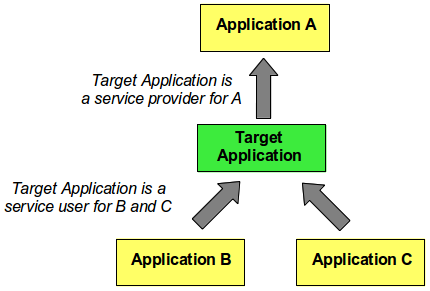
\includegraphics[scale=0.4,keepaspectratio=true]{ServConcept.png}
 \caption{Applications as Providers and Users of Services}
 \label{fig:ServConcept}
\end{figure}

The user of a service controls the service by sending \textit{commands} to the service provider. A command is a data exchange between a service user and a service provider to control the execution of a particular activity within the service provider. 

The provider of a service sends \textit{reports} to the user of the service. A report is a data exchange between a service provider (the report initiator) and a service user to provide information relating to the execution of a service activity.

Thus, a service consists of a set of commands which the user of the service sends to the provider of the service and of a set of reports which the service provider sends back to its user. A command defines actions to be executed by the service provider. 
A report encapsulates information about the internal state of the service provider (see figure \ref{fig:ServCmdRep}).

Against this background, the CORDET Framework of AD-1 fulfils two objectives:

\begin{fw_itemize}
\item{} It provides a formal definition of the abstract command concept and of the abstract report concept by building behavioural models of commands and reports which:
	\begin{fw_itemize}
	\item capture the aspects of the behaviour of commands and reports which is common to all commands and reports independently of the definition and implementation of a concrete command or report, and
	\item identify the adaptation points where service- and implementation-specific behaviour can be added.
	\end{fw_itemize}
\item{} It specifies the the component (the \textit{CORDET Components}) which implement the abstract command and report concepts.
\end{fw_itemize}

The CORDET Components cover, on the service user side, the sending of commands and the reception and distribution of reports and, on the service provider side, the processing of incoming commands and the generation of reports but do not cover the implementation of any concrete services. 

%--------------------------------------------------------------------------------
\subsubsection{Scope of PUS Extension of CORDET Framework}\label{sec:ScopePusExt}
Developers of a CORDET application are expected to deploy the CORDET components and complement them with application-specific components which implement the specific services of interest to them. The PUS extension of the CORDET Framework is intended to facilitate the task of application developers by offering them a set of pre-defined components which implement a set of \textit{Standard Services}. A standard service in this context is a service which implements commonly used functions within a certain domain. 

The standard services of the PUS Extension are taken from the Packet Utilization Standard (PUS) of AD-3. The target domain of the PUS Extension is therefore that of space-borne service-provider applications but it is worth stressing that the set of services selected from the PUS are those which are least dependent on the space context and it is therefore expected that the services implemented by the PUS Extension may be of interest to other application domains.

The standard services are defined by defining their commands and reports and the commands and reports are defined as specializations of the abstract command and report concepts of the CORDET Framework. Thus, a standard service is defined by “closing” the adaptation points identified in the abstract command and report concepts.

The CORDET Framework is ultimately intended to foster reuse (at both specification and implementation level) in the field of service-oriented embedded applications. The reuse model it promotes is illustrated in figure \ref{fig:HierarchicalDefServ}. 
At the top layer, there is the abstract definition of commands and reports of the CORDET Framework of AD-1. This definition is entirely generic and applicable to all services in all application. At the intermediate level, standard services are defined which capture concrete behaviour which is common to a large number of applications. The present document specifies one such set of standard services. Finally, at the bottom level, end-applications define their own services which are entirely specific to their needs. The application-level services may be either taken over from the standard services or they may be created as instantiations of the generic service concept (if they are entirely application-specific).

Note that the PUS Extension of the CORDET Framework specifies several services. These services are specified to be independent of each other so that the user may choose only a subset of these services. Similarly, each service is specified in terms of the commands and reports which implement it. Dependencies among the commands and reports of a service are minimized so that user may be free to import into their application just a subset of the commands and reports of a given service.

\begin{figure}[ht]
 \centering
 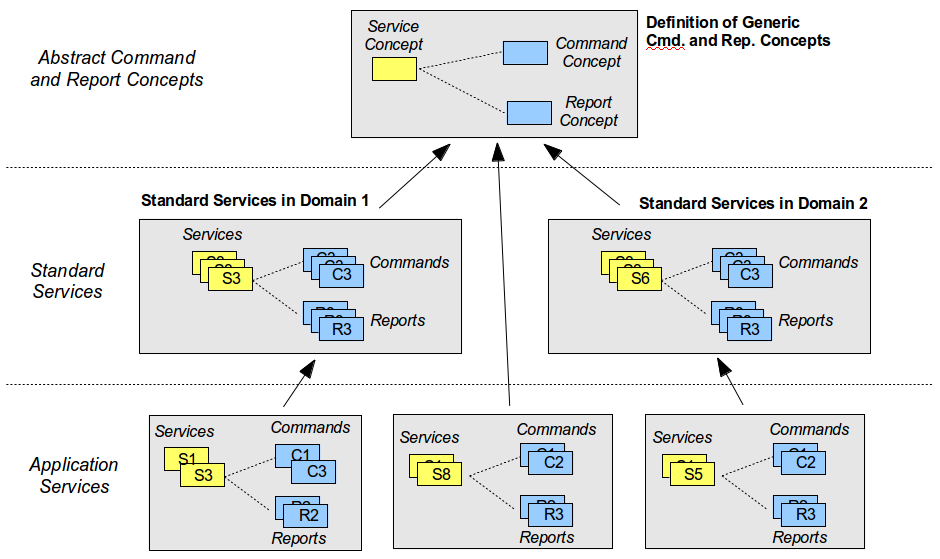
\includegraphics[scale=0.3,keepaspectratio=true]{HierarchicalDefServ.png}
 \caption{Hierarchical Definition of Services}
 \label{fig:HierarchicalDefServ}
\end{figure}


%---------------------------------------------------------------------------------
\subsubsection{Overview of Supported Services}
Table \ref{tab:supportedServ} lists the services supported by the PUS Extension of the CORDET Framework. The first column gives the service type identifier. The last column points to the section in this document where the support for the service is specified.

\begin{longtable}{|c|>{\raggedright\arraybackslash}p{6cm}|c|}
\caption{Services Supported by PUS Extension}\label{tab:supportedServ} \\
\hline
\rowcolor{light-gray}
\textbf{N} &\textbf{Service} & \textbf{Section} \\
\hline\hline
\endfirsthead
\rowcolor{light-gray}
\textbf{N} &\textbf{Service} & \textbf{Section} \\
\hline\hline
\endhead
1 & Request Verification Service & \ref{sec:serv1} \\
\hline
3 & Housekeeping Service & \ref{sec:serv3} \\
\hline
TBD & TBD & TBD \\
\hline
\end{longtable} 


%------------------------------------------------------------------------------------
\subsection{Specification Format} 
This document specifies the PUS Extension of the CORDET Framework. The framework is specified by defining its requirements. The requirements of the framework are of four types:

\begin{fw_itemize}
\item{} \textit{Standard Requirements} which define a desired feature of the framework extension. They are analogous in scope and format to the user requirements of a conventional (non-framework) application.
\item{} \textit{Adaptation Requirement} which define the points where a component offered by the framework extension can be extended by the application developers. 
In some cases, the definition of an adaptation point is accompanied by the definition of the default options offered by the framework extension for that adaptation point.  
\item{} \textit{Usage Constraint Requirements} which define the constraints on how the components offered by the framework extension may be used by application developers.
\item{} \textit{Property Requirements} which define behavioural properties which are guaranteed to hold on all applications which: (a) are instantiated from the CORDET Framework and its extension by closing their adaptation points, and (b) comply with the framework's usage constraints.
\end{fw_itemize}

To each framework requirement an \textit{identifier} is attached.
The requirement identifier takes the following form: x-y/t where 'x' is an acronym identifying the function to which the requirement applies; 'y' is a unique identifier within that function; and 't' identifies the requirement type. 
The type is designated by one single letter as follows: 'S' for the Standard Requirements, 'A' for the Adaptation Requirements, 'C' for the Usage Constraint Requirements and 'P' for the Property Requirements.

The specification of the framework extension includes a \textit{behavioural model} of the framework which describes its behaviour and identifies the adaptation points where application developers can extend this behaviour to match their requirements.  

The behavioural model of the framework extension is defined using the FW Profile of AD-2. 
It therefore consists of a set of \textit{state machines} (represented as state charts) and \textit{procedures} (represented as  activity diagrams). 
Familiarity with the FW Profile is essential for a full understanding of the framework requirements.

Wherever possible, the framework extension requirements simply make the state machines and procedures applicable. In other words, the state charts representing state machines and the activity diagrams representing procedures are treated as normative and no attempt is made to translate them into a comprehensive set of equivalent requirements.

In accordance with the FW Profile, the activity diagrams and state diagrams identify the framework adaptation points using the <<AP>> stereotype (but note that not all adaptation points are identified explicitly in activity or state diagrams). 
For convenience, all adaptation points with their default options are listed in dedicated tables. 
In most cases, the adaptation requirements simply make the items in such tables applicable. By default, the implementation mechanism for the adaptation points is left open and is not covered by this specification. 

Some of the components specified by the framework extension are defined as extensions of CORDET components. In such cases, the extended component is derived from the base component by either \textit{overriding} or \textit{closing} some of its adaptation points. 
A derived component overrides an adaptation point of its base component when it changes the default behaviour associated to that adaptation point (but applications can still change that behaviour). 
A derived component closes an adaptation point of its base component when it defines in a final way the behaviour associated to that adaptation point (i.e. applications can no longer change that behaviour).

%------------------------------------------------------------------------------------
\subsection{Command and Report Specification Format}\label{sec:CmdRepSpecFormat} 
Much of the specification of the PUS Extension of the CORDET Framework consists in the specification of the commands and reports which implement the selected PUS services. The CORDET Framework specifies the model of a generic command and a generic report and the PUS extension specializes these generic models to match the needs of the commands and reports implementing the selected PUS services. The specialization is done by closing or overriding the adaptation points identified in the generic command and report models.

The generic command and report model of the CORDET Framework defines a command or a report in terms of a set of \textit{attributes}, \textit{checks} and \textit{actions}.
Commands and reports are accordingly specified through tables with a format like that of tables \ref{sec:inCmdProc} and \ref{sec:outCmpProc}. The tables list the attributes, checks and actions or, respectively, commands and reports and they provide a specification of how these must be implemented for a particular command or report.




\begin{longtable}{|l|p{8.5cm}|}
\hline
\rowcolor{light-gray}
Name & $<$\textit{Name of Command}$>$ \\
\hline
Description & $<$\textit{Brief description of command}$>$ \\
\hline
Parameters & $<$\textit{Specification of parameters to be attached to command}$>$ \\
\hline
Synt. Check & $<$\textit{Specification of command-specific part of syntactical check to be executed to determine acceptance or rejection of command}$>$ \\
\hline
Ready Check & $<$\textit{Specification of command's Ready Check}$>$\\
\hline
Start Action & $<$\textit{Specification of command's Start Action}$>$ \\
\hline
Progress Action & $<$\textit{Specification of command's Progress Action}$>$\\
\hline
\end{longtable}

\begin{longtable}{{\raggedright\arraybackslash}p{4cm}|{\raggedright\arraybackslash}p{8cm}|}
\caption{Command Specification Table}\label{tab:cmdSpec} \\
\hline
\rowcolor{light-gray}
\textbf{N} &\textbf{Service} & \textbf{Section} \\
\hline\hline
\endfirsthead
\rowcolor{light-gray}
\textbf{N} &\textbf{Service} & \textbf{Section} \\
\hline\hline
\endhead
Name & $<$\textit{Name of Command}$>$ \\
\hline
Description & $<$\textit{Brief description of command}$>$ \\
\hline
Parameters & $<$\textit{Specification of parameters to be attached to command}$>$ \\
\hline
Synt. Check & $<$\textit{Specification of command-specific part of syntactical check to be executed to determine acceptance or rejection of command}$>$ \\
\hline
Ready Check & $<$\textit{Specification of command's Ready Check}$>$\\
\hline
Start Action & $<$\textit{Specification of command's Start Action}$>$ \\
\hline
Progress Action & $<$\textit{Specification of command's Progress Action}$>$\\
\hline
\end{longtable} 

%----------------------------------------------------------------------------------
\section{Compliance to PUS Requirements}\label{sec:ComplianceToPus}
The PUS Extension of the CORDET Framework implements a subset of the standard PUS services of AD-3. In order to provide visibility over the level of compliance to the PUS requirements of AD-3, appendix \ref{sec:PusReqSOC} presents a statement of compliance to these requirements. This demonstrates that, for the selected services, the PUS Extension is fully compliance to the PUS requirements.




%=============================================================================================
\section{The Data Pool Component}\label{sec:dp}
The Data Pool Component is a pre-defined component offered by the PUS Extension of the CORDET Framework. It is used by all services supported by the framework extension and it is therefore defined independently of these services.

%-----------------------------------------------------------------------------
\subsection{Data Pool Concepts}\label{sec:dpConcepts}
The Data Pool Component provides read-write access to a set of \textit{Data Items}. A Data Item is characterized by the following attributes: 

\begin{fw_itemize}
\item \textit{Default Value}: the value of the data item when the data pool is reset
\item \textit{Current Value}: the value of the data item at a particular point in time
\item \textit{Identifier}: a positive integer which uniquely identifies the Data Item within the Data Pool
\item \textit{Type}: an enumerated value which determines the range of possible values of the Data Item and its representation in the Data Pool
\end{fw_itemize}

With reference to the last bullet, it is noted that the set of supported types is defined at implementation level. The data items can be of two kinds:

\begin{fw_itemize}
\item \textit{Parameters}: data items whose value is under the control of an entity external to the host application 
\item \textit{Variables}: data items whose value is autonomously updated by the host application as part of its normal operation
\end{fw_itemize}

In practice, the data pool is the means through which a component can access data belonging to other components. Note that this specification is silent about the physical location of the data items in the data pool, which can be either the components which own the data item (in which case the data pool only offers a link to the data items), or the data pool itself, or a mixed solution where some data items reside in the data pool and others in peripheral components. 

This specification is similarly silent about the internal structure of data items and, in particular, it neither restricts them to be of primitive type nor does it mandate an array-like structure for them. Any such restrictions or options must be introduced at implementation level.

%---------------------------------------------------------------------------------
\section{Data Pool Behaviour}\label{sec:dpBehaviour}
The Data Pool Component - like all other CORDET Components - is an extension of the Base Component of section 3.2 of AD-1. It does not add any behaviour to the Base Component but it specializes some of its adaptation points as described below.

The Initialization Procedure of the Data Pool Components creates the data structures needed by the component. At one extreme, if an implementation chooses to locate all data items inside the Data Pool Component, then its Initialization Procedure is responsible for creating the data structures which host the data items. At the other extreme, in an implementation where data items remain located in their originating components and where the data pool only acts as a data switch-board, the Initialization Procedure does nothing and always returns "initialization successful".

When the Data Pool is reset, the current values of its data items are initialized with their default values. The Configuration Procedure is responsible for thus initializing the data item values. 

This specification does not say where the default values of the data items are stored in relation to their current values. At implementation level, two basic options are possible:

\begin{fw_enumerate}
\item The default values are stored alongside the current values
\item The default values are stored in some other memory area (e.g. in a EEPROM or in a remote location)
\end{fw_enumerate}

In the first case, the initialization of the data items simply involves a copy across two locations in RAM. in the second case, the initialization may be a potentially lengthy process involving the retrieval of the data items values from an external memory bank or from a remote location. The Data Pool Component covers both options and its Configuration Procedure is therefore defined as follows:

\begin{fw_itemize}
\item The Configuration Action starts the process whereby the default values of the data items are acquired and copied to their current values
\item The Configuration Check returns "success" if the initialization of the data item values can be done in zero logical time or else when the initialization has completed 
\end{fw_itemize}

Note that this logic implies that, in the case where the initialization of the data item values is not a zero logical time operation, then the Data Pool Component must be sent at least two Reset commands before it can enter the CONFIGURED state: the first Reset command starts the acquisition of the data item default values and the second Reset command verifies that their acquisition has been successful. Obviously, there is nothing to stop an application from using a "polling" approach and sending a sequence of Reset commands until the Data Pool Component has entered its CONFIGURED state.









\newpage
\appendix
%=============================================================================================
\section{PUS Requirements Compliance Matrix}\label{sec:PusReqSOC}
So




\end{document}  




